%\documentclass{article}
%\usepackage{graphicx,subfigure}
%\begin{document}

\begin{figure}[!h]
  \centering
  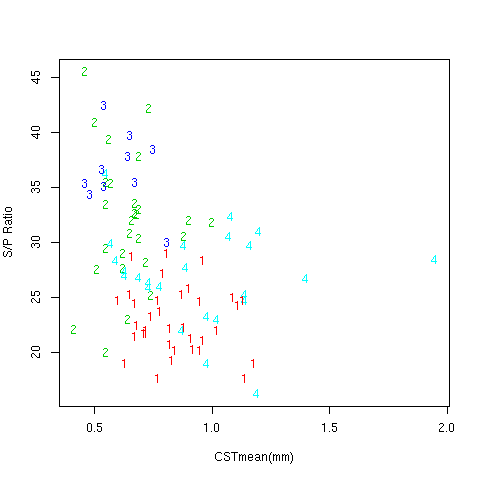
\includegraphics[width=1.0\textwidth]{spcstskin.png}
  \caption{Plot of CSTmean measurements against S/P ratio. The numbered points reveal the SkinType to which each data point belongs (1="flat", 2="semi-SRS", 3="SRS", 4="tight"). The correlation of these points is -0.38 which is significant at the 1 percent level for 106 observations}
  \label{fig:spcstskin}
\end{figure}

%\end{document}

